\documentclass{standalone}
\usepackage{tikz}
\usetikzlibrary{patterns, positioning}


\begin{document}
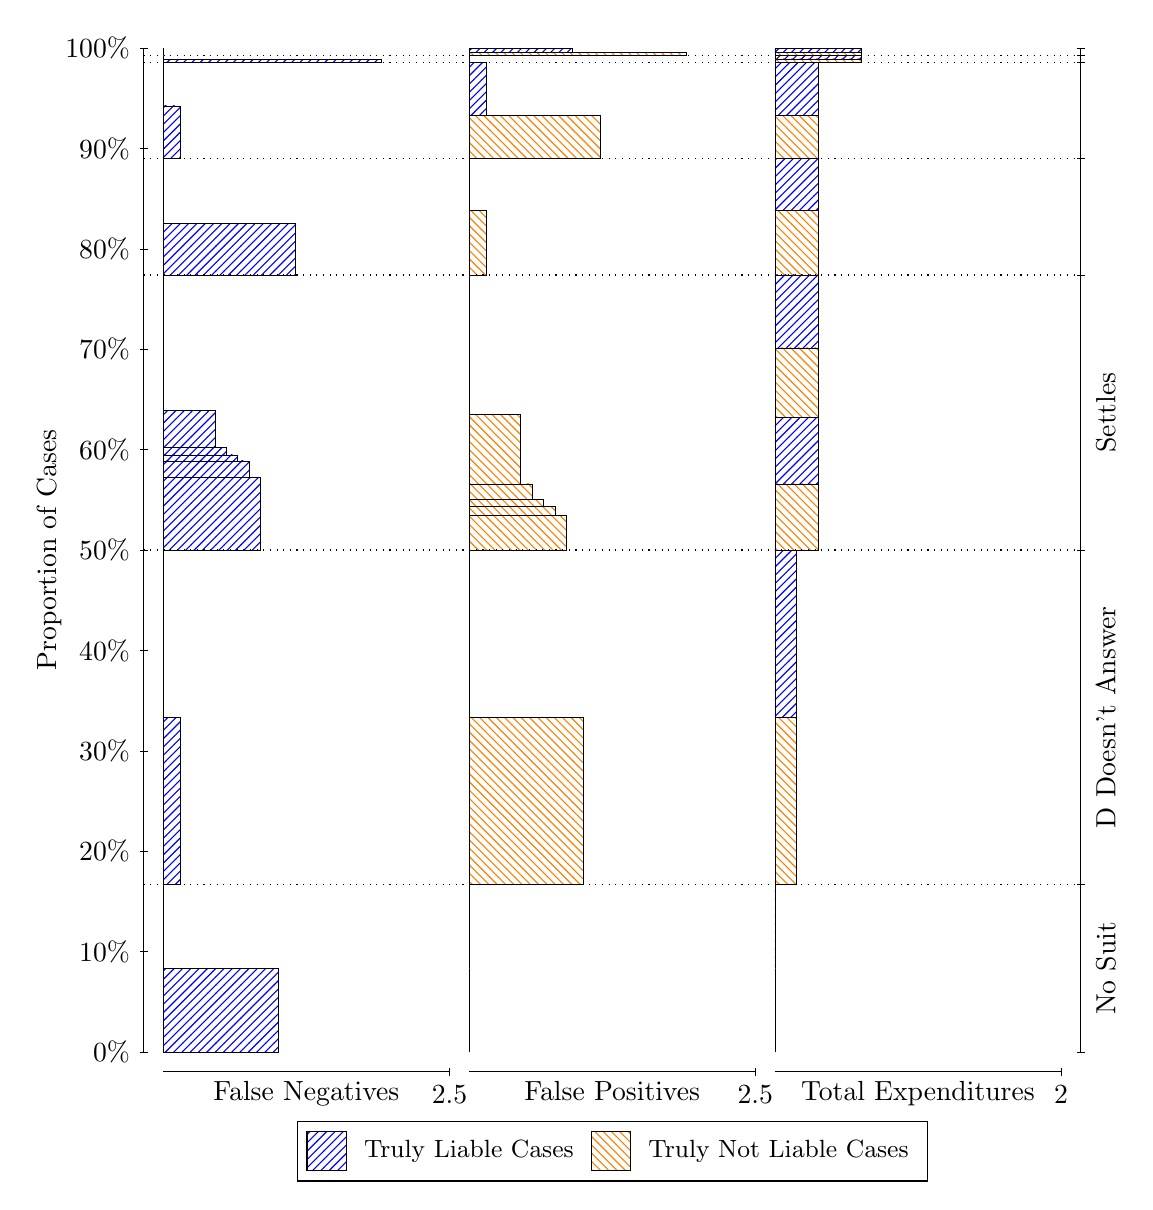
\begin{tikzpicture}
\draw[black, very thin] (1.5,1.75) -- (1.5,14.5);
\node[rotate=90, text=black, anchor=center] at (0.3, 8.125) {Proportion of Cases};
\draw[black, very thin] (1.45,1.75) -- (1.55,1.75);
\node[text=black, anchor=east] at (1.45, 1.75) {0\%};
\draw[black, very thin] (1.45,3.025) -- (1.55,3.025);
\node[text=black, anchor=east] at (1.45, 3.025) {10\%};
\draw[black, very thin] (1.45,4.3) -- (1.55,4.3);
\node[text=black, anchor=east] at (1.45, 4.3) {20\%};
\draw[black, very thin] (1.45,5.575) -- (1.55,5.575);
\node[text=black, anchor=east] at (1.45, 5.575) {30\%};
\draw[black, very thin] (1.45,6.85) -- (1.55,6.85);
\node[text=black, anchor=east] at (1.45, 6.85) {40\%};
\draw[black, very thin] (1.45,8.125) -- (1.55,8.125);
\node[text=black, anchor=east] at (1.45, 8.125) {50\%};
\draw[black, very thin] (1.45,9.4) -- (1.55,9.4);
\node[text=black, anchor=east] at (1.45, 9.4) {60\%};
\draw[black, very thin] (1.45,10.675) -- (1.55,10.675);
\node[text=black, anchor=east] at (1.45, 10.675) {70\%};
\draw[black, very thin] (1.45,11.95) -- (1.55,11.95);
\node[text=black, anchor=east] at (1.45, 11.95) {80\%};
\draw[black, very thin] (1.45,13.225) -- (1.55,13.225);
\node[text=black, anchor=east] at (1.45, 13.225) {90\%};
\draw[black, very thin] (1.45,14.5) -- (1.55,14.5);
\node[text=black, anchor=east] at (1.45, 14.5) {100\%};

\draw[black, very thin] (13.4,1.75) -- (13.4,14.5);
\draw[black, very thin] (13.35,1.75) -- (13.45,1.75);
\node[anchor=west] at (13.35, 1.75) {};
\draw[black, very thin] (13.35,3.875) -- (13.45,3.875);
\node[anchor=west] at (13.35, 3.875) {};
\draw[black, very thin] (13.35,8.125) -- (13.45,8.125);
\node[anchor=west] at (13.35, 8.125) {};
\draw[black, very thin] (13.35,11.618) -- (13.45,11.618);
\node[anchor=west] at (13.35, 11.618) {};
\draw[black, very thin] (13.35,13.094) -- (13.45,13.094);
\node[anchor=west] at (13.35, 13.094) {};
\draw[black, very thin] (13.35,14.313) -- (13.45,14.313);
\node[anchor=west] at (13.35, 14.313) {};
\draw[black, very thin] (13.35,14.406) -- (13.45,14.406);
\node[anchor=west] at (13.35, 14.406) {};
\draw[black, very thin] (13.35,14.5) -- (13.45,14.5);
\node[anchor=west] at (13.35, 14.5) {};

\draw[black, very thin, pattern color=blue, pattern=north east lines] (1.75,1.75) rectangle (3.2033,2.8125);
\draw[black, very thin, pattern color=orange, pattern=north west lines] (1.75,2.8125) rectangle (1.75,3.875);
\draw[black, very thin, pattern color=blue, pattern=north east lines] (1.75,3.875) rectangle (1.968,6);
\draw[black, very thin, pattern color=orange, pattern=north west lines] (1.75,6) rectangle (1.75,8.125);
\draw[black, very thin, pattern color=blue, pattern=north east lines] (1.75,8.125) rectangle (2.9853,9.0493);
\draw[black, very thin, pattern color=blue, pattern=north east lines] (1.75,9.0493) rectangle (2.84,9.2558);
\draw[black, very thin, pattern color=blue, pattern=north east lines] (1.75,9.2558) rectangle (2.6947,9.3338);
\draw[black, very thin, pattern color=blue, pattern=north east lines] (1.75,9.3338) rectangle (2.5493,9.4272);
\draw[black, very thin, pattern color=blue, pattern=north east lines] (1.75,9.4272) rectangle (2.404,9.8936);
\draw[black, very thin, pattern color=orange, pattern=north west lines] (1.75,9.8936) rectangle (1.75,11.618);
\draw[black, very thin, pattern color=blue, pattern=north east lines] (1.75,11.618) rectangle (3.4213,12.272);
\draw[black, very thin, pattern color=orange, pattern=north west lines] (1.75,12.272) rectangle (1.75,13.094);
\draw[black, very thin, pattern color=blue, pattern=north east lines] (1.75,13.094) rectangle (1.968,13.764);
\draw[black, very thin, pattern color=orange, pattern=north west lines] (1.75,13.764) rectangle (1.75,14.313);
\draw[black, very thin, pattern color=blue, pattern=north east lines] (1.75,14.313) rectangle (4.5113,14.356);
\draw[black, very thin, pattern color=orange, pattern=north west lines] (1.75,14.356) rectangle (1.75,14.406);
\draw[black, very thin, pattern color=orange, pattern=north west lines] (1.75,14.406) rectangle (1.75,14.449);
\draw[black, very thin, pattern color=blue, pattern=north east lines] (1.75,14.449) rectangle (1.75,14.5);
\draw[black, very thin, pattern color=orange, pattern=north west lines] (5.6333,1.75) rectangle (5.6333,2.8125);
\draw[black, very thin, pattern color=blue, pattern=north east lines] (5.6333,2.8125) rectangle (5.6333,3.875);
\draw[black, very thin, pattern color=orange, pattern=north west lines] (5.6333,3.875) rectangle (7.0867,6);
\draw[black, very thin, pattern color=blue, pattern=north east lines] (5.6333,6) rectangle (5.6333,8.125);
\draw[black, very thin, pattern color=orange, pattern=north west lines] (5.6333,8.125) rectangle (6.8687,8.5635);
\draw[black, very thin, pattern color=orange, pattern=north west lines] (5.6333,8.5635) rectangle (6.7233,8.6745);
\draw[black, very thin, pattern color=orange, pattern=north west lines] (5.6333,8.6745) rectangle (6.578,8.7634);
\draw[black, very thin, pattern color=orange, pattern=north west lines] (5.6333,8.7634) rectangle (6.4327,8.9635);
\draw[black, very thin, pattern color=orange, pattern=north west lines] (5.6333,8.9635) rectangle (6.2873,9.8492);
\draw[black, very thin, pattern color=blue, pattern=north east lines] (5.6333,9.8492) rectangle (5.6333,11.618);
\draw[black, very thin, pattern color=orange, pattern=north west lines] (5.6333,11.618) rectangle (5.8513,12.44);
\draw[black, very thin, pattern color=blue, pattern=north east lines] (5.6333,12.44) rectangle (5.6333,13.094);
\draw[black, very thin, pattern color=orange, pattern=north west lines] (5.6333,13.094) rectangle (7.3047,13.642);
\draw[black, very thin, pattern color=blue, pattern=north east lines] (5.6333,13.642) rectangle (5.8513,14.313);
\draw[black, very thin, pattern color=orange, pattern=north west lines] (5.6333,14.313) rectangle (5.6333,14.363);
\draw[black, very thin, pattern color=blue, pattern=north east lines] (5.6333,14.363) rectangle (5.6333,14.406);
\draw[black, very thin, pattern color=orange, pattern=north west lines] (5.6333,14.406) rectangle (8.3947,14.449);
\draw[black, very thin, pattern color=blue, pattern=north east lines] (5.6333,14.449) rectangle (6.9413,14.5);
\draw[black, very thin, pattern color=orange, pattern=north west lines] (9.5167,1.75) rectangle (9.5167,2.8125);
\draw[black, very thin, pattern color=blue, pattern=north east lines] (9.5167,2.8125) rectangle (9.5167,3.875);
\draw[black, very thin, pattern color=orange, pattern=north west lines] (9.5167,3.875) rectangle (9.7892,6);
\draw[black, very thin, pattern color=blue, pattern=north east lines] (9.5167,6) rectangle (9.7892,8.125);
\draw[black, very thin, pattern color=orange, pattern=north west lines] (9.5167,8.125) rectangle (10.062,8.9635);
\draw[black, very thin, pattern color=blue, pattern=north east lines] (9.5167,8.9635) rectangle (10.062,9.8078);
\draw[black, very thin, pattern color=orange, pattern=north west lines] (9.5167,9.8078) rectangle (10.062,10.693);
\draw[black, very thin, pattern color=blue, pattern=north east lines] (9.5167,10.693) rectangle (10.062,11.618);
\draw[black, very thin, pattern color=orange, pattern=north west lines] (9.5167,11.618) rectangle (10.062,12.44);
\draw[black, very thin, pattern color=blue, pattern=north east lines] (9.5167,12.44) rectangle (10.062,13.094);
\draw[black, very thin, pattern color=orange, pattern=north west lines] (9.5167,13.094) rectangle (10.062,13.642);
\draw[black, very thin, pattern color=blue, pattern=north east lines] (9.5167,13.642) rectangle (10.062,14.313);
\draw[black, very thin, pattern color=orange, pattern=north west lines] (9.5167,14.313) rectangle (10.607,14.363);
\draw[black, very thin, pattern color=blue, pattern=north east lines] (9.5167,14.363) rectangle (10.607,14.406);
\draw[black, very thin, pattern color=orange, pattern=north west lines] (9.5167,14.406) rectangle (10.607,14.449);
\draw[black, very thin, pattern color=blue, pattern=north east lines] (9.5167,14.449) rectangle (10.607,14.5);
\draw[black, dotted] (1.5,3.875) -- (13.4,3.875);
\draw[black, dotted] (1.5,8.125) -- (13.4,8.125);
\draw[black, dotted] (1.5,11.618) -- (13.4,11.618);
\draw[black, dotted] (1.5,13.094) -- (13.4,13.094);
\draw[black, dotted] (1.5,14.313) -- (13.4,14.313);
\draw[black, dotted] (1.5,14.406) -- (13.4,14.406);
\draw[black, very thin] (1.75,1.5) -- (5.3833,1.5);
\node[text=black, anchor=north] at (3.5667, 1.5) {False Negatives};
\draw[black, very thin] (5.3833,1.45) -- (5.3833,1.55);
\node[text=black, anchor=north] at (5.3833, 1.45) {2.5};

\draw[black, very thin] (5.6333,1.5) -- (9.2667,1.5);
\node[text=black, anchor=north] at (7.45, 1.5) {False Positives};
\draw[black, very thin] (9.2667,1.45) -- (9.2667,1.55);
\node[text=black, anchor=north] at (9.2667, 1.45) {2.5};

\draw[black, very thin] (9.5167,1.5) -- (13.15,1.5);
\node[text=black, anchor=north] at (11.333, 1.5) {Total Expenditures};
\draw[black, very thin] (13.15,1.45) -- (13.15,1.55);
\node[text=black, anchor=north] at (13.15, 1.45) {2};

\node[text=black, centered, rotate=90] at (13.72, 2.8125) {No Suit};
\node[text=black, centered, rotate=90] at (13.72, 6) {D Doesn't Answer};
\node[text=black, centered, rotate=90] at (13.72, 9.8714) {Settles};





\draw (7.449999999999999,1.5) node[draw=none] (baseCoordinate) {};
\begin{scope}[align=center]
        \matrix[scale=0.5, draw=black, below=0.5cm of baseCoordinate, nodes={draw}, column sep=0.1cm]{
            \node[rectangle, draw, minimum width=0.5cm, minimum height=0.5cm, pattern color=blue, pattern=north east lines] {}; &
            \node[draw=none, font=\small, text=black] (B) {Truly Liable Cases}; &
            \node[rectangle, draw, minimum width=0.5cm, minimum height=0.5cm, pattern color=orange, pattern=north west lines] {}; &
            \node[draw=none, font=\small, text=black] (B) {Truly Not Liable Cases}; \\
            };
\end{scope}

\end{tikzpicture}
\end{document}